\hypertarget{ux8a9eux6599ux4e2dux7684ux642dux914dux73feux8c61}{%
\chapter{語料中的搭配現象}\label{ux8a9eux6599ux4e2dux7684ux642dux914dux73feux8c61}}

語言是一個能夠攜帶並表達意義的系統。為了能傳達意義\ldots{}

一般來說,語言中的規律可以出現在任何一個語言單位上
(語音、詞素、字、詞彙、句子、篇章等)\footnote{因為語言不論在哪個單位\ldots{}},但傳統上,語料庫語言學關注的焦點是\textbf{詞彙}\ldots 要理解這兩種組合的差異相當簡單---我們知道礦泉水通常是以「瓶子」去盛裝,而較少以鍋子盛裝\footnote{當然,在現實世界中或許礦泉水\textbf{沒有}較\ldots{}}\ldots{}

上述所舉的例子在語言學中稱為\textbf{搭配語} \index{搭配語 (collocation)}
(collocation)。定義上\ldots:
\(p(瓶) \times p(礦泉水) = \frac{41}{50000} \times \frac{13}{50000} = 2.132 \times 10^{-7}\)
,「鍋」與「礦泉水」搭配出現的機率會是:
\(p(鍋) \times p(礦泉水) = \frac{39}{50000} \times \frac{13}{50000} = 2.028 \times 10^{-7}\)
。此時,我們便可以\textbf{將隨機排序當作基準}與\textbf{實際的資料}進行比較:

\begin{equation}\protect\hypertarget{eq:pmi1}{}{
\begin{aligned}
\frac{ p(瓶, 礦泉水) }{ p(瓶) p(礦泉水)} &= \frac{ 11/13 }{ 2.132 \times 10^{-7} } = 3968826.671 \\
\\
\frac{ p(鍋, 礦泉水) }{ p(鍋) p(礦泉水)} &= \frac{ 1/13 }{ 2.028 \times 10^{-7} } = 379305.113
\end{aligned}
}\label{eq:pmi1}\end{equation}

這些數值可以直觀地詮釋為\ldots{}

值得注意的是,搭配現象不只適用在詞彙單位上\ldots 至\textbf{構式}
\index{構式 (construction)} (construction)。

\hypertarget{ux8a5eux5f59ux4e4bux9593ux7684ux642dux914dux642dux914dux8a9e-collocation}{%
\section{詞彙之間的搭配:搭配語
(Collocation)}\label{ux8a5eux5f59ux4e4bux9593ux7684ux642dux914dux642dux914dux8a9e-collocation}}

\hypertarget{ux64cdux4f5cux5316ux642dux914dux73feux8c61ux5217ux806fux8868-contingency-table}{%
\subsection{操作化「搭配」現象:列聯表 (Contingency
Table)}\label{ux64cdux4f5cux5316ux642dux914dux73feux8c61ux5217ux806fux8868-contingency-table}}

舉例來說,下方的資料中共有 6 筆觀察值,記錄了 6
個人的資訊,並包含兩個類別變項 (1) \textbf{教育程度}以及 (2)
\textbf{性別}:

\begin{longtable}[]{@{}ccc@{}}
\toprule()
id & 教育程度 & 性別 \\
\midrule()
\endhead
1 & 國中 & 男 \\
2 & 高中職 & 女 \\
3 & 碩士 & 女 \\
4 & 大專 & 女 \\
5 & 大專 & 男 \\
6 & 高中職 & 男 \\
\bottomrule()
\end{longtable}

若想知道教育程度與性別有無關聯\ldots{}

\begin{longtable}[]{@{}ccccc@{}}
\toprule()
& 國中 & 高中職 & 大專 & 碩士 \\
\midrule()
\endhead
男 & 1 & 1 & 1 & 0 \\
女 & 0 & 1 & 0 & 2 \\
\bottomrule()
\end{longtable}

\hypertarget{ux642dux914dux8a9eux7684ux7a0bux5f0fux5be6ux4f5c}{%
\section{搭配語的程式實作}\label{ux642dux914dux8a9eux7684ux7a0bux5f0fux5be6ux4f5c}}

\hypertarget{ux7bc0ux9edeux8a5eux8207ux642dux914dux8a5e}{%
\subsection{節點詞與搭配詞}\label{ux7bc0ux9edeux8a5eux8207ux642dux914dux8a5e}}

前文在介紹搭配現象時,並未特別區分節點詞 (node word)
\index{節點詞 (node word)} 與搭配詞 (collocate)
\index{搭配詞 (collocate)} \ldots{}

\begin{figure}
\hypertarget{fig:ch07-sliding-window-0}{%
\centering
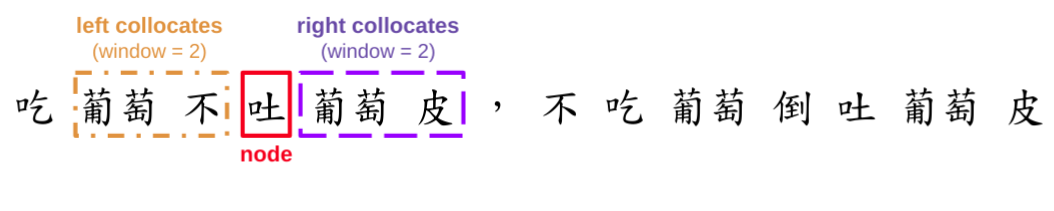
\includegraphics{figures/ch07_collocation_window.png}
\caption{節點詞與搭配詞}\label{fig:ch07-sliding-window-0}
}
\end{figure}

了解「節點詞/搭配詞」的定義後,我們以滑動窗口的演算法計算句中各種
\texttt{(節點詞,\ 搭配詞)} 組合出現的次數 (見
圖~\ref{fig:ch07-sliding-window})\ldots{}

\begin{figure}
\hypertarget{fig:ch07-sliding-window}{%
\centering
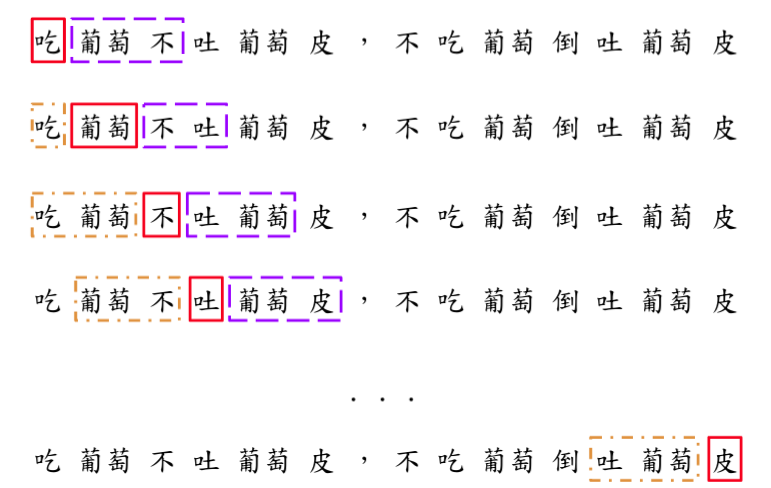
\includegraphics{figures/ch07_collocation_sliding_window.png}
\caption{以滑動窗口演算法計算句中「節點詞/搭配詞」組合次數}\label{fig:ch07-sliding-window}
}
\end{figure}

\begin{Shaded}
\begin{Highlighting}[]
\KeywordTok{def}\NormalTok{ count\_freq\_sent(sentence, left\_window, right\_window):}
\NormalTok{    cooccur\_freq }\OperatorTok{=}\NormalTok{ \{\} }\CommentTok{\# 共現頻率資料}
\NormalTok{    sent\_len }\OperatorTok{=} \BuiltInTok{len}\NormalTok{(sentence)}
    \ControlFlowTok{return}\NormalTok{ cooccur\_freq}
\end{Highlighting}
\end{Shaded}

在 \texttt{count\_freq\_sent()} 函數中,內層 for 迴圈的第三行是
\texttt{k\ =\ (node,\ collocate)}。因此,詞組內的第一個詞是節點詞,第二個詞是搭配詞,並非依照詞彙於句中出現的順序排列。例如:\texttt{(\textquotesingle{}葡萄\textquotesingle{},\ \textquotesingle{}吃\textquotesingle{})}
\ldots{}

在上方程式碼中,我們將左右窗口大小皆設為
2,因此搭配詞可能會出現在節點詞之前或之後。事實上,左右窗口的大小不一定要相同,依據目的不同,可以填入不一樣的左右窗口。舉例來說,有時候我們感興趣的是出現在節點詞\textbf{後方}的搭配詞\ldots{}

\hypertarget{ux91cfux5316ux642dux914dux5f37ux5f31}{%
\subsection{量化搭配強弱}\label{ux91cfux5316ux642dux914dux5f37ux5f31}}

我們要計算的列聯表如 表~\ref{tbl:collocation-contingency} 與
表~\ref{tbl:collocation-contingency-2}。\(O_{11}\)、\(O_{12}\)、\(O_{21}\)、\(O_{22}\)
為各種組合之下的頻率觀察值;\(R_{1}\)、\(R_{2}\)、\(C_{1}\)、\(C_{2}\)
則為邊際頻率 (marginal frequency)。

\hypertarget{tbl:collocation-contingency}{}
\begin{longtable}[]{@{}cccc@{}}
\caption{\label{tbl:collocation-contingency}節點詞/搭配詞列聯表
(實際頻率)}\tabularnewline
\toprule()
& Wc & \textasciitilde Wc & Total \\
\midrule()
\endfirsthead
\toprule()
& Wc & \textasciitilde Wc & Total \\
\midrule()
\endhead
Wn & \(O_{11}\) & \(O_{12}\) & \(R_{1}\) \\
\textasciitilde Wn & \(O_{21}\) & \(O_{22}\) & \(R_{2}\) \\
Total & \(C_{1}\) & \(C_{2}\) & N \\
\bottomrule()
\end{longtable}

\hypertarget{tbl:collocation-contingency-2}{}
\begin{longtable}[]{@{}
  >{\centering\arraybackslash}p{(\columnwidth - 6\tabcolsep) * \real{0.0658}}
  >{\centering\arraybackslash}p{(\columnwidth - 6\tabcolsep) * \real{0.4211}}
  >{\centering\arraybackslash}p{(\columnwidth - 6\tabcolsep) * \real{0.4211}}
  >{\centering\arraybackslash}p{(\columnwidth - 6\tabcolsep) * \real{0.0921}}@{}}
\caption{\label{tbl:collocation-contingency-2}節點詞/搭配詞列聯表
(頻率期望值)}\tabularnewline
\toprule()
\begin{minipage}[b]{\linewidth}\centering
\end{minipage} & \begin{minipage}[b]{\linewidth}\centering
Wc
\end{minipage} & \begin{minipage}[b]{\linewidth}\centering
\textasciitilde Wc
\end{minipage} & \begin{minipage}[b]{\linewidth}\centering
Total
\end{minipage} \\
\midrule()
\endfirsthead
\toprule()
\begin{minipage}[b]{\linewidth}\centering
\end{minipage} & \begin{minipage}[b]{\linewidth}\centering
Wc
\end{minipage} & \begin{minipage}[b]{\linewidth}\centering
\textasciitilde Wc
\end{minipage} & \begin{minipage}[b]{\linewidth}\centering
Total
\end{minipage} \\
\midrule()
\endhead
Wn & \(E_{11} = \frac{R_{1} C_{1}}{N}\) &
\(E_{12} = \frac{R_{1} C_{2}}{N}\) & \(R_{1}\) \\
\textasciitilde Wn & \(E_{21} = \frac{R_{2} C_{1}}{N}\) &
\(E_{22} = \frac{R_{2} C_{2}}{N}\) & \(R_{2}\) \\
Total & \(C_{1}\) & \(C_{2}\) & N \\
\bottomrule()
\end{longtable}

如果我們想知道 \texttt{(節點詞:電影,\ 搭配詞:日本)} 這個組合在
\texttt{corpus} 中的搭配情形,可以先列出以下列聯表:

\begin{equation}\protect\hypertarget{eq:association-measures}{}{
\begin{aligned}
MI       &= log2(\frac{O_{11}}{E_{11}}) \\
\\
\chi^2   &= \sum_{j} \frac{ (O_{j} - E_{j})^2 }{ E_{j} } \\
         &= \frac{ (O_{11} - E_{11})^2 }{ E_{11} } +
            \frac{ (O_{12} - E_{12})^2 }{ E_{12} } +
            \frac{ (O_{21} - E_{21})^2 }{ E_{21} } +
            \frac{ (O_{22} - E_{22})^2 }{ E_{22} } \\
\\
G^2      &= 2 \sum_{j}{O_{j}log\frac{O_{j}}{E_{j}}} \\
         &= 2 (O_{11}log\frac{O_{11}}{E_{11}} +
               O_{12}log\frac{O_{12}}{E_{12}} +
               O_{21}log\frac{O_{21}}{E_{21}} +
               O_{22}log\frac{O_{22}}{E_{22}})
\end{aligned}
}\label{eq:association-measures}\end{equation}

\hypertarget{ux69cbux5f0fux4e2dux7684ux642dux914dcollostruction}{%
\chapter{構式中的搭配:Collostruction}\label{ux69cbux5f0fux4e2dux7684ux642dux914dcollostruction}}

在前面的幾個段落裡,我們了解搭配語是出現在特定窗口大小
\index{窗口大小 (window size)}內的詞彙組。這個判斷方式已足以觀察到語料中一些穩定的現象,但卻未能利用語言的一項重要特性---語法關係
(syntactic relation) \index{語法關係 (syntactic relation)}\ldots{}

\hypertarget{ux95dcux65bc}{%
\section{關於}\label{ux95dcux65bc}}

在語料庫語言學裡,這方面的研究有兩個略有差異的方向。這個方向就是語料庫工具
\href{https://www.sketchengine.eu}{Sketch Engine} 中的詞彙素描 (word
sketch) 背後的基礎 (Huang et al., 2005; Kilgarriff et al., 2014;
Kilgarriff, Rychlý, Smrz, \& Tugwell,
2004),本書第八章有詳細介紹。第二個方向 (Gries \& Stefanowitsch, 2004;
Stefanowitsch \& Gries, 2005; Stefanowitsch \& Gries, 2003)
則是受\textbf{構式語法} (Construction Grammar)
\index{構式語法 (Construction Grammar)} (Goldberg, 1995)
的啟發,關注的是特定構式
\index{構式 (construction)}之下語法單位間的搭配關係。本章將著重介紹第二個方向。

\hypertarget{ux8cc7ux6599ux6e96ux5099}{%
\subsection{資料準備}\label{ux8cc7ux6599ux6e96ux5099}}

由於在搭配現象中引入了「語法」的概念,我們需要語法相關的資訊,亦即詞類標記
(part of speech, PoS) \index{詞類標記 (part of speech, PoS)}\ldots{}

\begin{Shaded}
\begin{Highlighting}[]
\ExtensionTok{pip}\NormalTok{ install }\AttributeTok{{-}U}\NormalTok{ ckiptagger[tf,gdown]}
\ExtensionTok{pip}\NormalTok{ install }\AttributeTok{{-}U}\NormalTok{ concordancer}
\end{Highlighting}
\end{Shaded}

\hypertarget{ux641cux5c0bux628aux5b57ux53e5}{%
\subsection{搜尋「把」字句}\label{ux641cux5c0bux628aux5b57ux53e5}}

有了剛剛的準備,我們便能開始從語料中搜尋抽象的\ldots{}

「把」字句的結構是「把 + (賓語) + (動作)」,例如,「把 \textbf{時間}
(賓語) \textbf{花} (動作) 在」。下方是「把」字句的 CQL
結構,\texttt{{[}{]}} 內是在描述該詞\ldots{}

上方這條搜尋語法裡面,定義了 3 個不同的 token:

\begin{enumerate}
\def\labelenumi{\arabic{enumi}.}
\tightlist
\item
  \texttt{{[}word="把"\ \&\ pos="P"{]}} 「把」這個詞(P
  介詞,詳見\href{https://github.com/ckiplab/ckiptagger/wiki/POS-Tags}{中研院詞類表})
\item
  \texttt{{[}pos="N{[}abcd{]}.*"{]}} 名詞(以 \texttt{Na/Nb/Nc/Nd}
  開頭的詞類)
\item
  \texttt{{[}pos="V.*"{]}} 動詞(所有以 \texttt{V} 開頭的詞類)
\end{enumerate}

語言複雜的程度總是超過我們的想像。事實上,上方的搜尋語法只能搜尋到\textbf{一部分的「把」字句},因為它忽略了其它的可能,例如「\textbf{把}
寶貴 的 \textbf{時間} \textbf{花} 在」這個把字句不符\ldots{}

\hypertarget{ux53c8ux662fux4e00ux7ae0}{%
\chapter{又是一章}\label{ux53c8ux662fux4e00ux7ae0}}

\hypertarget{ux7c21ux4ecb}{%
\section{簡介}\label{ux7c21ux4ecb}}

接下來,讓我們利用「把」字句的資料進行構式中的搭配分析 (Collostruction
Analysis)。以下將會介紹三種量化方式,分別為 Collexeme Analysis
(Stefanowitsch \& Gries, 2003)、Covarying Collexeme Analysis
(Stefanowitsch \& Gries, 2005),以及 Distinctive Collexeme Analysis
(Gries \& Stefanowitsch, 2004)。

\hypertarget{ux69cbux5f0fux8207ux8a5eux5f59ux7684ux4e92ux76f8ux5438ux5f15}{%
\subsection{構式與詞彙的互相吸引}\label{ux69cbux5f0fux8207ux8a5eux5f59ux7684ux4e92ux76f8ux5438ux5f15}}

Collexeme Analysis 用於衡量構式與其空槽 (lexical slot)
內的詞彙的共現傾向。例如:可以藉由此種分析方式得知什麼詞彙特別容易做為\textbf{賓語}出現在「把」字句中。Collexeme
Analysis 透過列聯表量化構式與詞彙互相吸引的程度。以
表~\ref{tbl:collexeme-analysis1} 為例,透過此列\ldots{}

\hypertarget{tbl:collexeme-analysis1}{}
\begin{longtable}[]{@{}cccc@{}}
\caption{\label{tbl:collexeme-analysis1}「把字句」(構式) 與「錢」(賓語)
的列聯表}\tabularnewline
\toprule()
& 錢 & \textasciitilde 錢 & Total \\
\midrule()
\endfirsthead
\toprule()
& 錢 & \textasciitilde 錢 & Total \\
\midrule()
\endhead
把字句 & \(O_{11}\) & \(O_{12}\) & \(R_{1}\) \\
\textasciitilde 把字句 & \(O_{21}\) & \(O_{22}\) & \(R_{2}\) \\
Total & \(C_{1}\) & \(C_{2}\) & \(N\) \\
\bottomrule()
\end{longtable}

要計算出 表~\ref{tbl:collexeme-analysis1}
內每個項目的頻率,除了搜尋得來的「把」字句的共現環境 (concordance)
之外,還需要一些額外的資訊。首先,\texttt{concordancer}
所找出的把字句筆數,即是 表~\ref{tbl:collexeme-analysis1} 的 \(R_{1}\)
,而 \(O_{11}\) 則是賓語「錢」在這些把字句中出現的頻率。透過 \(R_{1}\)
與 \(O_{11}\) ,即可以算出 \(O_{12}\),也就是 \(R_{1}\) -
\(O_{11}\)。\(C_{1}\) 則\ldots{}

\begin{Shaded}
\begin{Highlighting}[]
\NormalTok{\{}
    \StringTok{\textquotesingle{}L1\textquotesingle{}}\NormalTok{: \{ }\StringTok{\textquotesingle{}o11\textquotesingle{}}\NormalTok{: freq, }\StringTok{\textquotesingle{}all\textquotesingle{}}\NormalTok{: freq \},}
    \StringTok{\textquotesingle{}L2\textquotesingle{}}\NormalTok{: \{ }\StringTok{\textquotesingle{}o11\textquotesingle{}}\NormalTok{: freq, }\StringTok{\textquotesingle{}all\textquotesingle{}}\NormalTok{: freq \},}
    \StringTok{\textquotesingle{}L3\textquotesingle{}}\NormalTok{: \{ }\StringTok{\textquotesingle{}o11\textquotesingle{}}\NormalTok{: freq, }\StringTok{\textquotesingle{}all\textquotesingle{}}\NormalTok{: freq \},}
\NormalTok{    ...}
\NormalTok{\}}
\end{Highlighting}
\end{Shaded}

\hypertarget{ux69cbux5f0fux4e4bux4e2dux7684ux8a5eux5f59ux642dux914dcovarying-collexeme-analysis}{%
\subsection{構式之中的詞彙搭配:Covarying Collexeme
Analysis}\label{ux69cbux5f0fux4e4bux4e2dux7684ux8a5eux5f59ux642dux914dcovarying-collexeme-analysis}}

衡量同一句式下的兩個 lexical slots 內的詞彙的共現傾向 e.g.,
「把」字句中的賓語與動作,如:把 時間(slot1) 花(slot2) 在\ldots{}

\hypertarget{ux91cfux5316ux76f8ux4f3cux69cbux5f0fux4e4bux9593ux7684ux5deeux7570distinctive-collexeme-analysis}{%
\subsection{量化相似構式之間的差異:Distinctive Collexeme
Analysis}\label{ux91cfux5316ux76f8ux4f3cux69cbux5f0fux4e4bux9593ux7684ux5deeux7570distinctive-collexeme-analysis}}

比較兩種 (or 多種) 句式中,相應位置之 lexical slot 的偏好 e.g.,
「把」字句 vs.「將」字句,句中之動詞使用偏好

\hypertarget{custom-box}{%
\subsection{Custom Box}\label{custom-box}}

\begin{mybox}{自訂區塊標題}

這是 \textbf{Box} 裡面的\emph{段落}。這是 Box 裡面的段落。這是 Box
裡面的段落。這是 Box 裡面的段落。這是 Box 裡面的段落。這是 Box
裡面的段落。這是 Box 裡面的段落。這是 Box 裡面的段落。

Markdown content and other blocks are enabled, e.g., code:

\begin{Shaded}
\begin{Highlighting}[]
\BuiltInTok{print}\NormalTok{(}\StringTok{"Custom code block"}\NormalTok{)}
\end{Highlighting}
\end{Shaded}

這是 Box 裡面的段落。這是 Box 裡面的段落。這是 Box 裡面的段落。這是 Box
裡面的段落。這是 Box 裡面的段落。這是 Box 裡面的段落。This is a custom
block. This is a custom block. This is a custom block.

\end{mybox}

\appendix

\hypertarget{r-ux57faux790e}{%
\chapter{R 基礎}\label{r-ux57faux790e}}

R
語言是從統計社群開發出來的語言,比較傑出的地方在於統計相關的計算與製圖。近年來由於幾位知名的語言學家的大力推廣,使
R 語言成為語料庫語言學研究的主流程式語言之一。開源的開發環境 RStudio
的出現,更是使得R語言的編程與專案協作,甚至與 web app (shiny)
的開發工作更加便利迅速。R語言社群對於資料處理的套件開發速度也相當驚人,還有許多進階的統計計算與作圖套件方便研究者從事量化的語音與文本分析。

\hypertarget{ux5411ux91cf}{%
\section{向量}\label{ux5411ux91cf}}

R 以向量(vector)當作基本單位,在Python中的「一個變數的回傳值」,在 R
中的概念其實是「一個長度為 1 的向量」。而 R 的 vector 又分成 6
種類別,其中較常見的 4 種為 \texttt{integer}, \texttt{double},
\texttt{character}, \texttt{logical}。

\begin{enumerate}
\def\labelenumi{\arabic{enumi}.}
\tightlist
\item
  integer vector 的元素由整數組成,可以是零、正數或負數。

  \begin{itemize}
  \tightlist
  \item
    除了使用\texttt{:} 製造數列,也可以使用 \texttt{c()} (稱為
    concatenate) 組出任意序列的 vector。
  \item
    使用 \texttt{c()} 製造 integer vector 時,每個整數數字後面必須接
    \texttt{L},若沒有加上 \texttt{L}, R 會將製造出來的 vector 視為
    double vector。
  \end{itemize}
\item
  double vector 的元素由浮點數組成,亦即含有小數點的數字 (e.g 1.2,
  -0.75)

  \begin{itemize}
  \tightlist
  \item
    double vector 和 integer vector 合稱 numeric
    vector,通常不太需要區別兩者,因為 R
    在運算時,會將這兩種資料類型自動轉換成合適的類型。
  \end{itemize}
\item
  character vector 的每個元素皆由一個字串組成。

  \begin{itemize}
  \tightlist
  \item
    R 也可以儲存字串 (string)。在 R 裡面,只要是被引號 (quote, ' 或 ''
    皆可) 包裹的東西就是字串,放在引號內的可以是任何字元
    (e.g.~空白、數字、中文字、英文字母)。
  \item
    如果字串內含有引號 ``,需在字串內的引號前使用跳脫字元
    ,以表示此引號是字串的一部分而非字串的開頭或結尾。也可以使用「不同的」引號,弱勢以「單引號」表示字串的開頭與結尾時,字串內就可以直接使用「雙引號」,反之亦然。
  \end{itemize}
\item
  logical vector 的每個元素由 TRUE 或 FALSE 組成。

  \begin{itemize}
  \tightlist
  \item
    可以使用 c() 一項項手動輸入製造 logical vector,另一個來源則是
    logical test 的回傳值:
  \item
    boolean operators (\&, \textbar, !, any(), all()) 可以整合多個
    logical tests
  \item
    logical operators: ==, !=, \textgreater, \textless, \%in\%
  \end{itemize}
\end{enumerate}

在 R 運算兩個或兩個以上的 vector 時,通常以 element-wise 的方式進行。若
vector 長度不相同,例如\texttt{c(1,\ 2,\ 3)\ +\ 2}, R 會自動將長度較短
vector (2) 回收(recycle),也就是重複此向量內的元素,拉長到與另一個
vector 等長,再將兩個一樣長的 vector 進行 element-wise
的向量運算。vector 內的每個元素,其資料類型(data
type)必須相同。資料類型即是前面提到的 integer, double, character,
logical。若資料類型不一致(例如:將不同資料類型的元素放入 c()),R
會根據某些規則,自動進行資料類型的轉換。

\hypertarget{ux5411ux91cfux4e2dux7684ux5143ux7d20}{%
\subsection{向量中的元素}\label{ux5411ux91cfux4e2dux7684ux5143ux7d20}}

我們可以透過 3 種方式來取出 vector 裡的元素,傳回一個新的
vector。第一種方式是透過元素在 vector 中的位置次序 (index):

\begin{Shaded}
\begin{Highlighting}[]
\CommentTok{\# LETTERS 是 R 內建變數: 一個包含所有大寫英文字母的 character vector}

\NormalTok{LETTERS[}\DecValTok{1}\NormalTok{]}
\CommentTok{\#\textgreater{} [1] "A"}

\NormalTok{LETTERS[}\DecValTok{1}\SpecialCharTok{:}\DecValTok{5}\NormalTok{]}
\CommentTok{\#\textgreater{} [1] "A" "B" "C" "D" "E"}

\NormalTok{LETTERS[}\FunctionTok{c}\NormalTok{(}\DecValTok{1}\NormalTok{, }\DecValTok{3}\NormalTok{, }\DecValTok{5}\NormalTok{)]}
\CommentTok{\#\textgreater{} [1] "A" "C" "E"}
\end{Highlighting}
\end{Shaded}

\hypertarget{ux524dux8655ux7406ux8207-stringr-ux5957ux4ef6}{%
\section{前處理與 stringr
套件}\label{ux524dux8655ux7406ux8207-stringr-ux5957ux4ef6}}

正如本書第三章介紹在 Python 的文字前處理方式,我們也可以使用 R
來進行。透過各程式語言通用的 Regex 以及 R 的 stringr
套件,我們可以撰寫合適的 function 來清理語料。

我們先來認識 stringr 這個套件。它是 tidyverse
套件中負責處理字串的套件,比起 base R 的字串處理函數,stringr
中的函數名稱較一致(str\_*)。在 R 裡面,Regex
是以字串(character)的資料類型來表徵,因此需注意:若是 Regex
包含反斜線,則需要在每一個反斜線之前再加上一個反斜線。舉例來說,在
Python 我們要跳過\texttt{.}這個字元時,會寫作
\texttt{today\textbackslash{}.\$},但在 R
中就必須寫成\texttt{today\textbackslash{}\textbackslash{}.\$}。

\texttt{str\_detect()} 是一個常用的 stringr 函數。若是我們想知道向量
\texttt{s\ \textless{}-\ c("cat",\ "bed",\ "car",\ "Mr.")}
中,哪些元素擁有字串 a 時,就可以使用
\texttt{str\_detect(s,\ "a")},則程式會回傳一個logical vector
\texttt{{[}1{]}\ \ TRUE\ FALSE\ \ TRUE\ FALSE}。\texttt{str\_detect()}也可結合
{[} {]} 或 dplyr 套件中的 filter() 函數,來篩選出元素的值:

\begin{Shaded}
\begin{Highlighting}[]
\NormalTok{s }\OtherTok{\textless{}{-}} \FunctionTok{c}\NormalTok{(}\StringTok{"cat"}\NormalTok{, }\StringTok{"bed"}\NormalTok{, }\StringTok{"car"}\NormalTok{, }\StringTok{"Mr."}\NormalTok{)}
\NormalTok{s[}\FunctionTok{str\_detect}\NormalTok{(s, }\StringTok{"\^{}c"}\NormalTok{)]}

\CommentTok{\#\textgreater{} [1] "cat" "car"}
\end{Highlighting}
\end{Shaded}

\hypertarget{ux4e2dux6587ux6587ux672cux8cc7ux6599ux8655ux7406}{%
\section{中文文本資料處理}\label{ux4e2dux6587ux6587ux672cux8cc7ux6599ux8655ux7406}}

\hypertarget{ux65b7ux8a5e}{%
\subsection{斷詞}\label{ux65b7ux8a5e}}

jieba 是一個用於中文斷詞的 Python 套件。jiebaR 則是 jieba 的 R
版本。透過 jiebaR 進行斷詞只需要兩個步驟:使用 \texttt{worker()}
初始化斷詞設定,再使用 \texttt{segment()}
將文字斷詞。\texttt{jiebaR::segment()} 會回傳一個 character
vector,vector 內的每個元素都是一個被斷出來的詞:

\begin{Shaded}
\begin{Highlighting}[]
\FunctionTok{library}\NormalTok{(jiebaR)}
\NormalTok{seg }\OtherTok{\textless{}{-}} \FunctionTok{worker}\NormalTok{()}
\NormalTok{txt }\OtherTok{\textless{}{-}} \StringTok{"失業的熊讚陪柯文哲看銀翼殺手"} 
\FunctionTok{segment}\NormalTok{(txt, seg)}

\CommentTok{\#\textgreater{} [1] "失業" "的熊" "讚" "陪" "柯文" "哲看" "銀翼" "殺手"}
\end{Highlighting}
\end{Shaded}

遇到專有名詞或是特殊詞彙時,jiebaR
的斷詞可能會不太精準。若想避免這種情況,可以新增一份自訂辭典(儲存在一份純文字檔,每個詞佔一行),例如我們的自訂辭典
\texttt{user\_dict.txt} 的內容如下:

\hypertarget{tidytext-ux5957ux4ef6}{%
\subsection{tidytext 套件}\label{tidytext-ux5957ux4ef6}}

至於 tidytext 則是一個較近期的 text mining 套件,它將 tidyverse
的想法運用到文本資料處理,換言之,它使用 data frame
的資料結構去表徵和處理文本資料。若是我們使用 tidytext
處理文本資料,能在文本分析的過程中結合 dplyr 與
ggplot2,快速地視覺化文本資料。

不過在 tidytext framework
之下,文章的內部(詞彙與詞彙之間的)結構會消失,因為一段文本對於
tidytext 來說就是 bag-of-words。由於 tidytext 儲存文本資料的格式是
one-token-per-document-per-row,在一個 data frame 中,每個row
是一篇文章中的一個 token。舉例來說,如果我們有兩篇文章,第一篇被斷成 38
個詞彙,第二篇被斷成 20 個詞彙,則我們總共需要一個擁有 58 rows 的 data
frame 來儲存這兩篇文章。

一般而言,tidytext 的架構適合詞頻相關的分析,像是計算文章的 lexical
diversity,或是透過詞頻進行情緒分析。透過
\texttt{tidytext::unnest\_tokens()},我們可以將 \texttt{docs\_df}
儲存的文本資料(已斷詞),變成 tidytext format,也就是
one-token-per-document-per-row 的 data

\hypertarget{ux5411ux91cfux8868ux5fb5}{%
\section{向量表徵}\label{ux5411ux91cfux8868ux5fb5}}

由於資料科學以及統計學方法上的限制,我們要對文本進行量化分析之前,常常要將原本以符碼
(文字)
表徵的文本轉成數值表徵,才能對文本進行相似度計算、分群、分類等等分析。將文本轉換成數值的表徵方式相當多,其中一種最簡單的方式,即是使用
document-term matrix 將文本以數值向量去表徵。

\begin{Shaded}
\begin{Highlighting}[]
\CommentTok{\#\textquotesingle{} doc1:    "I baked the cake and the muffin"}
\CommentTok{\#\textquotesingle{} doc2:    "I loved the cake"}
\CommentTok{\#\textquotesingle{} doc3:    "I wrote the book"}
\CommentTok{\#\textquotesingle{} TERMS:        I  baked loved wrote the and cake muffin book}
\NormalTok{dtm }\OtherTok{\textless{}{-}} \FunctionTok{matrix}\NormalTok{(}\FunctionTok{c}\NormalTok{( }\DecValTok{1}\NormalTok{,   }\DecValTok{1}\NormalTok{,    }\DecValTok{0}\NormalTok{,    }\DecValTok{0}\NormalTok{,   }\DecValTok{2}\NormalTok{,  }\DecValTok{1}\NormalTok{,   }\DecValTok{1}\NormalTok{,    }\DecValTok{1}\NormalTok{,   }\DecValTok{0}\NormalTok{ ,}
                 \DecValTok{1}\NormalTok{,   }\DecValTok{0}\NormalTok{,    }\DecValTok{1}\NormalTok{,    }\DecValTok{0}\NormalTok{,   }\DecValTok{1}\NormalTok{,  }\DecValTok{0}\NormalTok{,   }\DecValTok{1}\NormalTok{,    }\DecValTok{0}\NormalTok{,   }\DecValTok{0}\NormalTok{ , }
                 \DecValTok{1}\NormalTok{,   }\DecValTok{0}\NormalTok{,    }\DecValTok{0}\NormalTok{,    }\DecValTok{1}\NormalTok{,   }\DecValTok{1}\NormalTok{,  }\DecValTok{0}\NormalTok{,   }\DecValTok{0}\NormalTok{,    }\DecValTok{0}\NormalTok{,   }\DecValTok{1}\NormalTok{ ), }
              \AttributeTok{nrow =} \DecValTok{3}\NormalTok{, }\AttributeTok{ncol =} \DecValTok{9}\NormalTok{, }\AttributeTok{byrow =} \ConstantTok{TRUE}\NormalTok{)}

\NormalTok{dtm}
\CommentTok{\#\textgreater{}      [,1] [,2] [,3] [,4] [,5] [,6] [,7] [,8] [,9]}
\CommentTok{\#\textgreater{} [1,]    1    1    0    0    2    1    1    1    0}
\CommentTok{\#\textgreater{} [2,]    1    0    1    0    1    0    1    0    0}
\CommentTok{\#\textgreater{} [3,]    1    0    0    1    1    0    0    0    1}
\end{Highlighting}
\end{Shaded}

有了文本的向量表徵之後,我們就能去量化比較文本之間的相似度,方法是直接利用向量之間的距離公式
\(d(\overrightarrow{p}, \overrightarrow{q})\) 以及相似度公式
\(cos(\theta)\):

\[
d(\overrightarrow{p}, \overrightarrow{q}) = \sqrt{ (p_1 - q_1)^2 + (p_2 - q_2)^2 + ... + (p_n - q_n)^2 }
\]

\[
cos(\theta) = \frac{\overrightarrow{p} \cdot \overrightarrow{q}}{\lVert p \rVert \lVert q \rVert }
\]

\hypertarget{latent-semantic-anlysis-dimensionality-reduction}{%
\subsection{Latent Semantic Anlysis (Dimensionality
Reduction)}\label{latent-semantic-anlysis-dimensionality-reduction}}

由於 document-term matrix 通常很稀疏,很多值會是
0,使文本向量無法抓到某些文本之間的語意關聯。比如 doc2 與 doc4
雖然語意相近,但此二文本的向量的相似度 (cosine similarity)
為零,因為這兩篇文本並未使用到相同的詞彙。面對這種情形,我們可以將高維的
document-term matrix
透過數學方式轉換成維度比較小的矩陣。在這個過程中,document-term matrix
中一些語意相近的詞彙會被壓縮到某個或是某些維度中,讓這個維度比較小的矩陣反而比較能表徵文本之間的語意關聯。這種方式稱為
Latent Semantic Analysis (LSA),而用來將矩陣分解降維的數學方法稱為
Singular Value Decomposition (SVD)。

\begin{Shaded}
\begin{Highlighting}[]
\NormalTok{lsa\_model }\OtherTok{\textless{}{-}}\NormalTok{ quanteda.textmodels}\SpecialCharTok{::}\FunctionTok{textmodel\_lsa}\NormalTok{(q\_dfm, }\AttributeTok{nd =} \DecValTok{15}\NormalTok{)}
\FunctionTok{dim}\NormalTok{(lsa\_model}\SpecialCharTok{$}\NormalTok{docs)}
\CommentTok{\#\textgreater{} [1] 300  15}

\CommentTok{\# Document similarity}
\NormalTok{doc\_sim2 }\OtherTok{\textless{}{-}} \FunctionTok{textstat\_simil}\NormalTok{(}\FunctionTok{as.dfm}\NormalTok{(lsa\_model}\SpecialCharTok{$}\NormalTok{docs), }\AttributeTok{method =} \StringTok{"cosine"}\NormalTok{)}
\FunctionTok{sort}\NormalTok{(doc\_sim2[}\StringTok{"anti\_1.txt"}\NormalTok{, ], }\AttributeTok{decreasing =}\NormalTok{ T)[}\DecValTok{1}\SpecialCharTok{:}\DecValTok{8}\NormalTok{]}
\CommentTok{\#\textgreater{}   anti\_1.txt    pro\_2.txt anti\_102.txt anti\_146.txt   pro\_94.txt   pro\_84.txt }
\CommentTok{\#\textgreater{}    1.0000000    0.9963039    0.9959590    0.9936474    0.9933724    0.9933206 }
\CommentTok{\#\textgreater{}  anti\_94.txt  pro\_133.txt }
\CommentTok{\#\textgreater{}    0.9923490    0.9921601}
\end{Highlighting}
\end{Shaded}

\hypertarget{ux53c3ux8003ux6587ux737b}{%
\chapter*{參考文獻}\label{ux53c3ux8003ux6587ux737b}}
\addcontentsline{toc}{chapter}{參考文獻}

\hypertarget{refs}{}
\begin{CSLReferences}{1}{0}
\leavevmode\vadjust pre{\hypertarget{ref-goldberg1995}{}}%
Goldberg, A. E. (1995). \emph{Constructions : A construction grammar
approach to argument structure}. {Chicago}: {University of Chicago
Press}.

\leavevmode\vadjust pre{\hypertarget{ref-gries2004}{}}%
Gries, S. Th., \& Stefanowitsch, A. (2004). Extending collostructional
analysis: {A} corpus-based perspective on `alternations\&apos;
\emph{International Journal of Corpus Linguistics}, \emph{9}(1),
97--129. Journal Article. \url{https://doi.org/10.1075/ijcl.9.1.06gri}

\leavevmode\vadjust pre{\hypertarget{ref-huang2005}{}}%
Huang, C.-R., Kilgarriff, A., Wu, Y., Chiu, C.-M., Smith, S., Rychlỳ,
P., \ldots{} Chen, K.-J. (2005). Chinese {Sketch Engine} and the
extraction of grammatical collocations. In \emph{Proceedings of the
fourth {SIGHAN} workshop on {Chinese} language processing}.

\leavevmode\vadjust pre{\hypertarget{ref-kilgarriff2014}{}}%
Kilgarriff, A., Baisa, V., Bušta, J., Jakubíček, M., Kovář, V.,
Michelfeit, J., \ldots{} Suchomel, V. (2014). The {Sketch Engine}: Ten
years on. \emph{Lexicography}, \emph{1}(1), 7--36.
\url{https://doi.org/10.1007/s40607-014-0009-9}

\leavevmode\vadjust pre{\hypertarget{ref-kilgarriff2004}{}}%
Kilgarriff, A., Rychlý, P., Smrz, P., \& Tugwell, D. (2004). The {Sketch
Engine}. In G. Williams \& S. Vessier (Eds.), \emph{Proceedings of the
11th {EURALEX} international congress} (pp. 105--115). {Lorient,
France}: {Université de Bretagne-Sud, Faculté des lettres et des
sciences humaines}.

\leavevmode\vadjust pre{\hypertarget{ref-stefanowitsch2005}{}}%
Stefanowitsch, A., \& Gries, S. T. (2005). Covarying collexemes.
\emph{Corpus Linguistics and Linguistic Theory}, \emph{1}(1), 1--43.
\url{https://doi.org/10.1515/cllt.2005.1.1.1}

\leavevmode\vadjust pre{\hypertarget{ref-stefanowitsch2003}{}}%
Stefanowitsch, A., \& Gries, S. Th. (2003). Collostructions:
{Investigating} the interaction of words and constructions.
\emph{International Journal of Corpus Linguistics}, \emph{8}(2),
209--243. Journal Article. \url{https://doi.org/10.1075/ijcl.8.2.03ste}

\end{CSLReferences}
